%%%%%%%%%%%%%%%%%%%%%%%%%%%%%%%%%%%%%%%%%
%%% HYPERRIDE Reporting Template
%%%%%%%%%%%%%%%%%%%%%%%%%%%%%%%%%%%%%%%%%

\documentclass[letterpaper,12pt]{report}
\usepackage[pass]{geometry}
\usepackage{istgame}
\usepackage{xcolor}
\usepackage{xurl}
\usepackage{hyperride}		% HYPERRIDE specific definitions and styles  
\usepackage[utf8]{inputenc}	% UTF8 package
\usepackage[T1]{fontenc}
\usepackage{textcomp}		% common special chars
\usepackage{amsmath}		% math formula
\usepackage{fancybox}
\usepackage{anyfontsize}	% fonts
\usepackage{lipsum}
\usepackage{float}
\usepackage[normalem]{ulem}
\usepackage{cleveref}
\usepackage[printonlyused]{acronym}
\hypersetup{
	pdftitle={Beacon Labs - Workshop},
	pdfauthor={[Dylan Gresham, Jordan Whyte, Gunnar Vittrup, Josh Boyle, Gaby Dagher]},
	pdfkeywords={Beacon Labs, Workshop, Cybersecurity, Middlebox, TCP Amplification, Network Security, Mobile Security, Web Security, Service Workers, XSS, Cross-Site Scripting, Android Vulnerability},
}
\usepackage{booktabs}
\usepackage{subfigure}
\usepackage{graphicx}
\usepackage{xcolor}
\usepackage{soul}
\sethlcolor{lightgray}
\usepackage[export]{adjustbox}
\usepackage{mdframed}
\usepackage{pdfpages}
\usepackage{comment}
\usepackage{multirow,array}
\def\todo#1{{\color{hyperridered}\textbf{TODO:} ``#1''}}
\def\hyperride{HYPERRIDE}
\definecolor{lightblue}{rgb}{0.87, 0.94, 1}
\graphicspath{ {graphics/} }

%%%%%%%%%%%%%%%%%%%%%%%%%%%%%%%%%%%%%%%%%
%%% Definitions
%%%%%%%%%%%%%%%%%%%%%%%%%%%%%%%%%%%%%%%%%

%% stuff for displaying code

% Define the listing package
\usepackage{listings} % code highlighter
\usepackage{color} % use color
\definecolor{mygreen}{rgb}{0,0.6,0}
\definecolor{mygray}{rgb}{0.5,0.5,0.5}
\definecolor{mymauve}{rgb}{0.58,0,0.82}

% Customize a bit the look
\lstset{ %
  backgroundcolor=\color{white}, % choose the background color; you must add \usepackage{color} or \usepackage{xcolor}
  basicstyle=\footnotesize, % the size of the fonts that are used for the code
  breakatwhitespace=false, % sets if automatic breaks should only happen at whitespace
  breaklines=true, % sets automatic line breaking
  captionpos=b, % sets the caption-position to bottom
  commentstyle=\color{mygreen}, % comment style
  deletekeywords={...}, % if you want to delete keywords from the given language
  escapeinside={\%*}{*)}, % if you want to add LaTeX within your code
  extendedchars=true, % lets you use non-ASCII characters; for 8-bits encodings only, does not work with UTF-8
  frame=tblr, % adds a frame around the code with line numbers inside the box
  keepspaces=true, % keeps spaces in text, useful for keeping indentation of code (possibly needs columns=flexible)
  keywordstyle=\color{blue}, % keyword style
  % language=Octave, % the language of the code
  morekeywords={*,...}, % if you want to add more keywords to the set
  numbers=left, % where to put the line-numbers; possible values are (none, left, right)
  numbersep=5pt, % how far the line-numbers are from the code
  numberstyle=\tiny\color{mygray}, % the style that is used for the line-numbers
  rulecolor=\color{black}, % if not set, the frame-color may be changed on line-breaks within not-black text (e.g. comments (green here))
  showspaces=false, % show spaces everywhere adding particular underscores; it overrides 'showstringspaces'
  showstringspaces=false, % underline spaces within strings only
  showtabs=false, % show tabs within strings adding particular underscores
  stepnumber=1, % the step between two line-numbers. If it's 1, each line will be numbered
  stringstyle=\color{mymauve}, % string literal style
  tabsize=2, % sets default tabsize to 2 spaces
  title=\lstname % show the filename of files included with \lstinputlisting; also try caption instead of title
}
% END of listing package %

\definecolor{darkgray}{rgb}{.4,.4,.4}
\definecolor{purple}{rgb}{0.65, 0.12, 0.82}

% Define Javascript language
\lstdefinelanguage{JavaScript}{
  keywords={typeof, new, true, false, catch, function, return, null, catch, switch, var, if, in, while, do, else, case, break},
  keywordstyle=\color{blue}\bfseries,
  ndkeywords={class, export, boolean, throw, implements, import, this},
  ndkeywordstyle=\color{darkgray}\bfseries,
  identifierstyle=\color{black},
  sensitive=false,
  comment=[l]{//},
  morecomment=[s]{/*}{*/},
  commentstyle=\color{purple}\ttfamily,
  stringstyle=\color{red}\ttfamily,
  morestring=[b]',
  morestring=[b]"
}

\lstset{
  language=JavaScript,
  extendedchars=true,
  basicstyle=\footnotesize\ttfamily,
  showstringspaces=false,
  showspaces=false,
  numbers=left,
  numberstyle=\footnotesize,
  numbersep=9pt,
  tabsize=2,
  breaklines=true,
  showtabs=false,
  captionpos=b
}

%%%%%%%%%%%%%%%%%%%%%%%%%%%%%%%%%%%%%%%%%
%%% Definitions
%%%%%%%%%%%%%%%%%%%%%%%%%%%%%%%%%%%%%%%%%
\newcounter{taskset}
\setcounter{taskset}{1} % Set the initial value of the taskset counter

\newcounter{action}[taskset]
\renewcommand{\theaction}{\thesection.\arabic{taskset}.\arabic{action}}

\newcommand{\myaction}[1]{%
  \refstepcounter{action}%
  \textbf{Action \theaction: #1}%
}


% CHANGE %'s below to make subsection headings visible/invisible in TOC
%\newcommand{\xsubsubsection}[1]{\subsection{#1}}
%\newcommand{\xsubsubsection}[1]{\subsubsection{#1}}

\setcounter{secnumdepth}{4}
\setcounter{tocdepth}{5}

\begin{document}


\includepdf[pages=1]{./graphics/2FP.pdf}

\mdfdefinestyle{code}{%
    linecolor=black,
    outerlinewidth=2pt,
    %roundcorner=20pt,
    innertopmargin=4pt,
    innerbottommargin=4pt,
    innerrightmargin=4pt,
    innerleftmargin=4pt,
    leftmargin = 4pt,
    rightmargin = 4pt
    backgroundcolor=black!10
}

\setcounter{tocdepth}{4}
\setcounter{secnumdepth}{4}

%%%%%%%%%%%%%%%%%%%%%%%%%%%%%%%%%%%%%%%%%
%%% URL style same as regular text
%%%%%%%%%%%%%%%%%%%%%%%%%%%%%%%%%%%%%%%%%
	
\urlstyle{same}

%%%%%%%%%%%%%%%%%%%%%%%%%%%%%%%%%%%%%%%%%
%%% Deliverable Information
%%%%%%%%%%%%%%%%%%%%%%%%%%%%%%%%%%%%%%%%%

% Project Meta Information
\ProjectFullTitle{Beacon Network Security Labs: Middlebox Amplification Attack Activity}
\ProjectAcronym{HYPERRIDE}
\ProjectRefNo{957788}

% Report Number, use either "1", "2", or "3" for the corresponding reporting period
\delivNumber{0}

% Period covered by the report
\delivFrom{dd/mm/yyyy}
\delivTo{dd/mm/yyyy}

% Report Responsible Partner
\delivResponsible{AIT Austrian Institute of Technology (AIT)} 

% Report Version, Contractual and Actual Date, Dissemination Level, Type
\delivVersion{vn.n}
\ContractualDate{dd/mm/yyyy}
\ActualDate{dd/mm/yyyy}

% List of Main Authors (usually from the responsible partner)
\delivAuthor{[Dylan Gresham, Gaby Dagher]}

% List of Co-Authors (all other co-authors should be listed here)
\delivFPAuthor{[]}

% Report Status
\delivStatus{d} %% d = draft, f = final, s = submitted

%%%%%%%%%%%%%%%%%%%%%%%%%%%%%%%%%%%%%%%%%
%%% Change Log
%%%%%%%%%%%%%%%%%%%%%%%%%%%%%%%%%%%%%%%%%

\istChange{dd/mm/yyyy}{v1.0}{Name (Partner short name)}{Draft report template}
\istChange{}{}{}{}

%%%%%%%%%%%%%%%%%%%%%%%%%%%%%%%%%%%%%%%%%
%%% Cover Page
%%%%%%%%%%%%%%%%%%%%%%%%%%%%%%%%%%%%%%%%%

%\makecover

%%%%%%%%%%%%%%%%%%%%%%%%%%%%%%%%%%%%%%%%%
%%% Table of Contents
%%%%%%%%%%%%%%%%%%%%%%%%%%%%%%%%%%%%%%%%%

\clearpage
\fancypagestyle{plain}{}
\settableofcontents
\tableofcontents
\clearpage

%%%%%%%%%%%%%%%%%%%%%%%%%%%%%%%%%%%%%%%%%
%%% Overview
%%%%%%%%%%%%%%%%%%%%%%%%%%%%%%%%%%%%%%%%%
\newpage

section*{Virtual Machine Setup}\label{sec:Virtual-Machine-Setup}
\addcontentsline{toc}{section}{Virtual Machine Setup}

\subsection*{Virtual Machine Software Installation}\label{sec:Virtual-Machine-Software-Installation}
\addcontentsline{toc}{subsection}{Virtual Machine Software Installation}

VirtualBox will be the virtual machine software that is used to open the VM images and complete the activity. It is possible to complete the activity with other virtual machine software but it has been untested and so support for other virtual machine software will not be included in this workshop document at this point in time.

Begin by downloading Oracle's VirtualBox software version 7.0.18. The download links for VirtualBox can be found at the below \href{https://www.virtualbox.org/wiki/Download_Old_Builds_7_0}{website}. If you already have a newer version of VirtualBox installed, you should be able to follow the same steps.

\url{https://www.virtualbox.org/wiki/Download_Old_Builds_7_0}

\subsubsection*{Windows Setup}\label{sec:Virtual-Machine-Windows-Setup}
\addcontentsline{toc}{subsubsection}{Windows Setup}

\paragraph*{Steps:}

\begin{enumerate}
    \item Select the hyperlink titled ``Windows hosts'' under the ``VirtualBox x.x.xx platform packages'' as seen in Figure~\ref{fig:win-1} to begin the installation of the latest version of VirtualBox. This activity was created when VirtualBox 7.0.18 was the latest release, however, the steps provided should still apply to future versions of VirtualBox as well.

    \begin{figure}[!htbp]
        \centering
        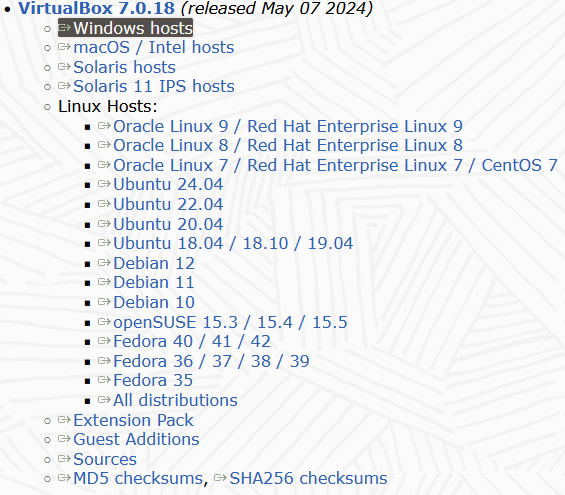
\includegraphics[width=0.75\linewidth]{graphics/Windows_VBox_Install_1.png}
        \caption{Download button is highlighted in gray for Windows machines.}
        \label{fig:win-1}
    \end{figure}
    
    \item Once the download has completed, run the downloaded installer. The file name should be ``VirtualBox-<version\_number>-Win.exe''.
    \item Run through the installer without changing anything. At the end, make sure the checkbox is selected to ``Start Oracle VM VirtualBox x.x.xx after installation'' as shown in Figure~\ref{fig:win-2} then click the ``Finish'' button to complete the installation and open VirtualBox.

    \begin{figure}[!htbp]
        \centering
        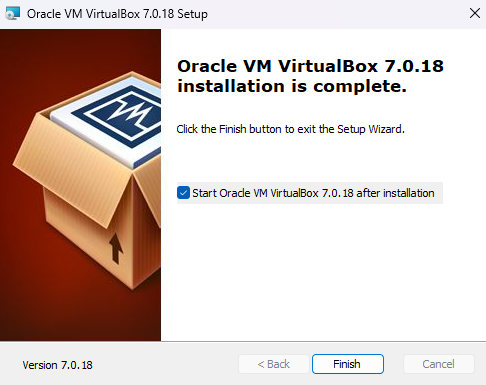
\includegraphics[width=0.75\linewidth]{graphics/Windows_VBox_Install_2.png}
        \caption{Final screen for the Windows installer.}
        \label{fig:win-2}
    \end{figure}
    
    \item Once VirtualBox has been installed and opened, please continue to the ``Downloading and Importing the Images'' section.
\end{enumerate}

\newpage
\subsubsection*{Linux Setup}\label{sec:Virtual-Machine-Linux-Setup}
\addcontentsline{toc}{subsubsection}{Linux Setup}

\begin{enumerate}
    \item From the VirtualBox download page seen in Figure~\ref{fig:win-1}, find your distribution of Linux and follow the instructions Oracle has provided.
    \item If your distribution isn't shown on the website, please look into distribution specific instructions for your Linux distro. For example, if you are using Arch Linux, there is a VirtualBox page on the ArchWiki that provides an installation guide.
\end{enumerate}

\newpage
\subsection*{Downloading and Importing the Images}
\addcontentsline{toc}{subsection}{Downloading and Importing the Images}

This activity will be done using two virtual machines that will be provided to you. The image files for this activity's VM can be found in the following \href{https://drive.google.com/drive/folders/19hjc2iZTGFC1OyWLpr8P4DVq1M6V3B9-?usp=sharing}{Google Drive folder}, full link shown below.

\url{https://drive.google.com/drive/folders/19hjc2iZTGFC1OyWLpr8P4DVq1M6V3B9-?usp=sharing}

\paragraph*{Steps:}

\begin{enumerate}
    \item Use the above link to open the Google Drive folder containing the two virtual machine image files.
    \item Download both image files. The files are 7.79 and 8.61 GB in size so the download may take a while.
    \item Once the images have been downloaded, they can be imported into VirtualBox by navigating to File > Import Appliance and selecting the .ova image files that were downloaded. Only one .ova file can be selected and imported at a time. Visual instructions can be seen in Figures~\ref{fig:import-appliance}, \ref{fig:import-file-button}, \ref{fig:import-file-picker}, \ref{fig:import-after-file-picker}, and~\ref{fig:import-finish}.

    \begin{figure}[!htbp]
        \centering
        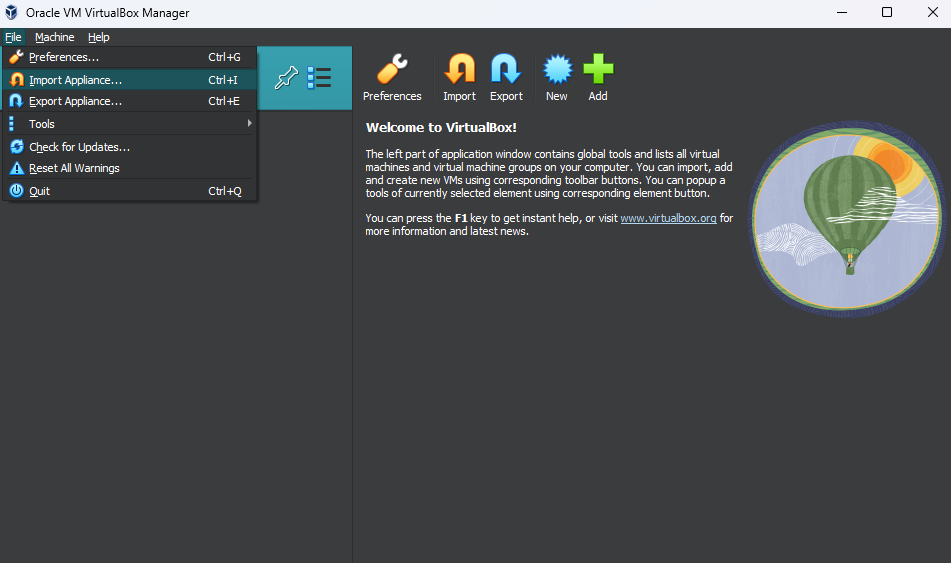
\includegraphics[width=0.75\linewidth]{graphics/import-appliance.png}
        \caption{File > Import Appliance}
        \label{fig:import-appliance}
    \end{figure}
    
    \begin{figure}[!htbp]
        \centering
        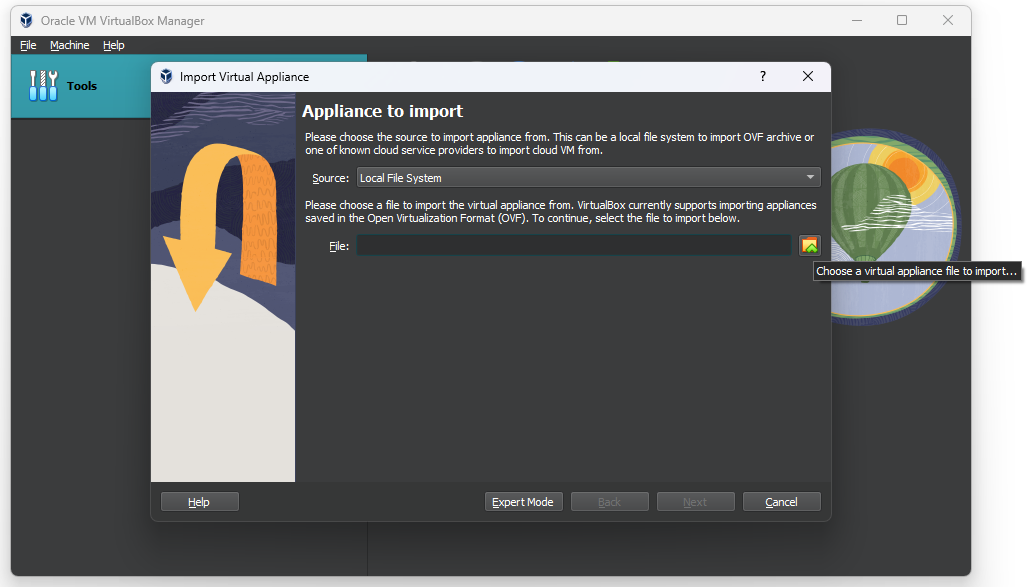
\includegraphics[width=0.75\linewidth]{graphics/import-file-button.png}
        \caption{Select the file button to choose one of the downloaded image file.}
        \label{fig:import-file-button}
    \end{figure}
    
    \begin{figure}[!htbp]
        \centering
        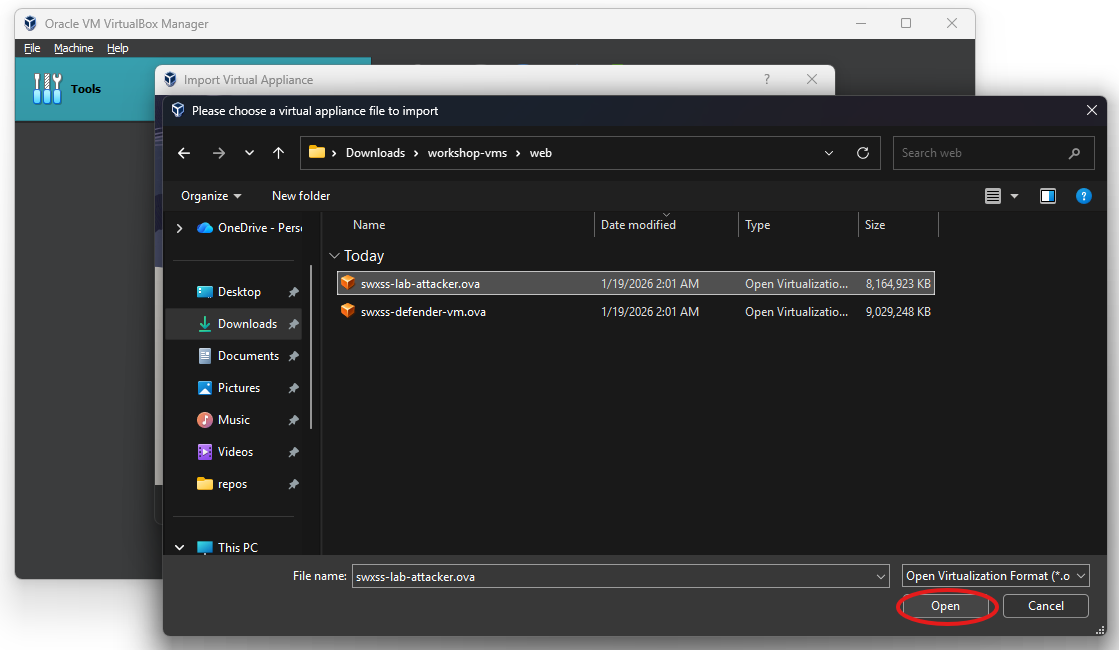
\includegraphics[width=0.75\linewidth]{graphics/import-file-picker.png}
        \caption{Choose one of the downloaded .ova files to import.}
        \label{fig:import-file-picker}
    \end{figure}
    
    \begin{figure}[!htbp]
        \centering
        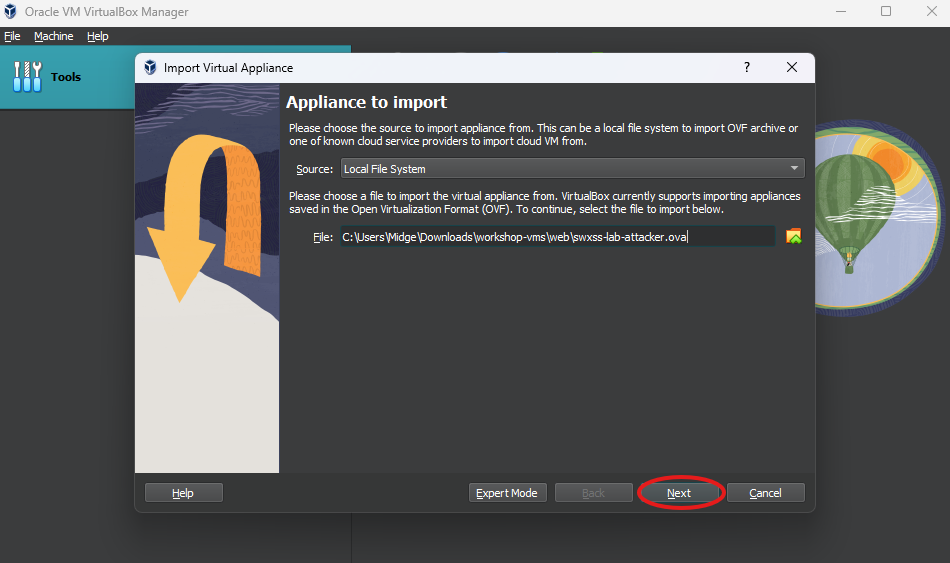
\includegraphics[width=0.75\linewidth]{graphics/import-after-filepicker.png}
        \caption{Select next after selecting the image to import.}
        \label{fig:import-after-file-picker}
    \end{figure}
    
    \begin{figure}[!htbp]
        \centering
        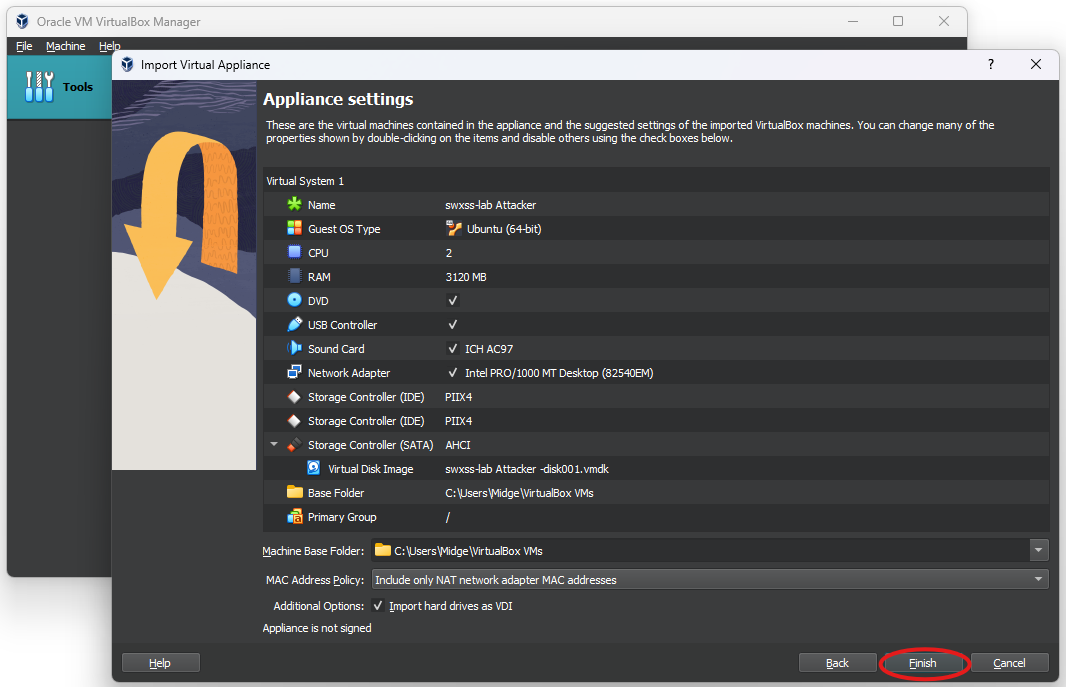
\includegraphics[width=0.75\linewidth]{graphics/import-finish.png}
        \caption{Final confirmation. Your file paths and names may differ slightly.}
        \label{fig:import-finish}
    \end{figure}
    
    \item Repeat steps 2 and 3 with the other image file.
    \item Once both images have been imported to VirtualBox, continue to the final section, ``Verifying Import.''
\end{enumerate}

\subsection*{Verifying Import}
\addcontentsline{toc}{subsection}{Verifying Import}

\paragraph*{Steps:}

\begin{enumerate}
    \item Before starting the virtual machines, verify that both images are on the ``swxss-network'' as seen in Figure~\ref{fig:verify-network}. If one or both machines are not on this network, skip to Step 6 and then come back here after.

    \begin{figure}[!htbp]
        \centering
        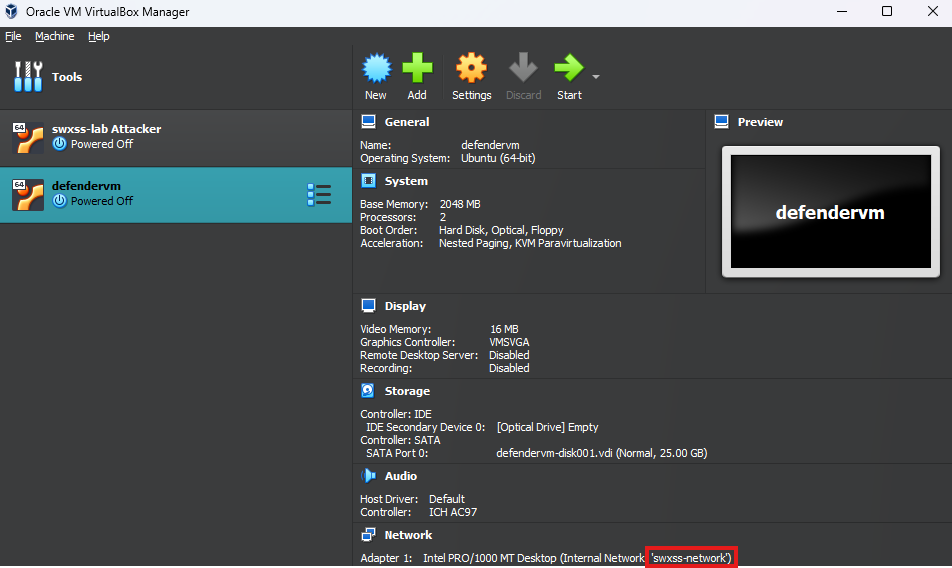
\includegraphics[width=0.75\linewidth]{graphics/verify-network.png}
        \caption{Ensure that the Network is an Internal Network titled ``swxss-network.''}
        \label{fig:verify-network}
    \end{figure}
    
    \item Start the ``defendervm'' virtual machine by selecting it and clicking the green ``Start'' button. The defender vm can be started in the headless state, shown in Figure~\ref{fig:headless-start}, if desired.

    \begin{figure}[!htbp]
        \centering
        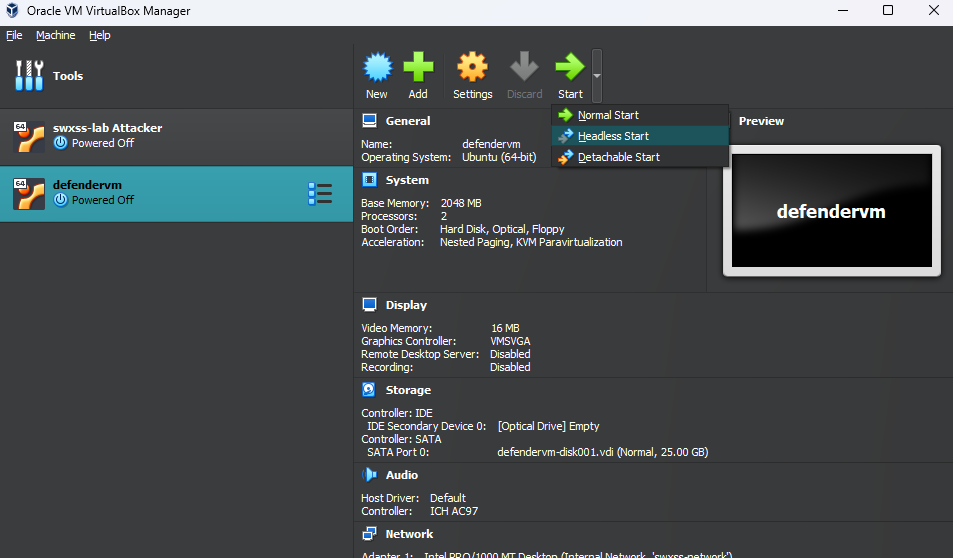
\includegraphics[width=0.75\linewidth]{graphics/headless-start.png}
        \caption{The defender vm can be started in a headless state to have less windows cluttering your desktop.}
        \label{fig:headless-start}
    \end{figure}
    
    \item Start the ``swxss-lab Attacker'' virtual machine by selecting it and clicking the green ``Start'' button.
    \item Within the attacker virtual machine, using the username and password ``swxss'' log in and open up the Firefox browser.
    \item Enter the url \url{https://www.swxss.com/dom-example.php#context=Mary}. If greeted with a the Main Dashboard for Mary as seen in Figure~\ref{fig:verify-success} skip to Step 7, otherwise continue on to the next step.

    \begin{figure}[!htbp]
        \centering
        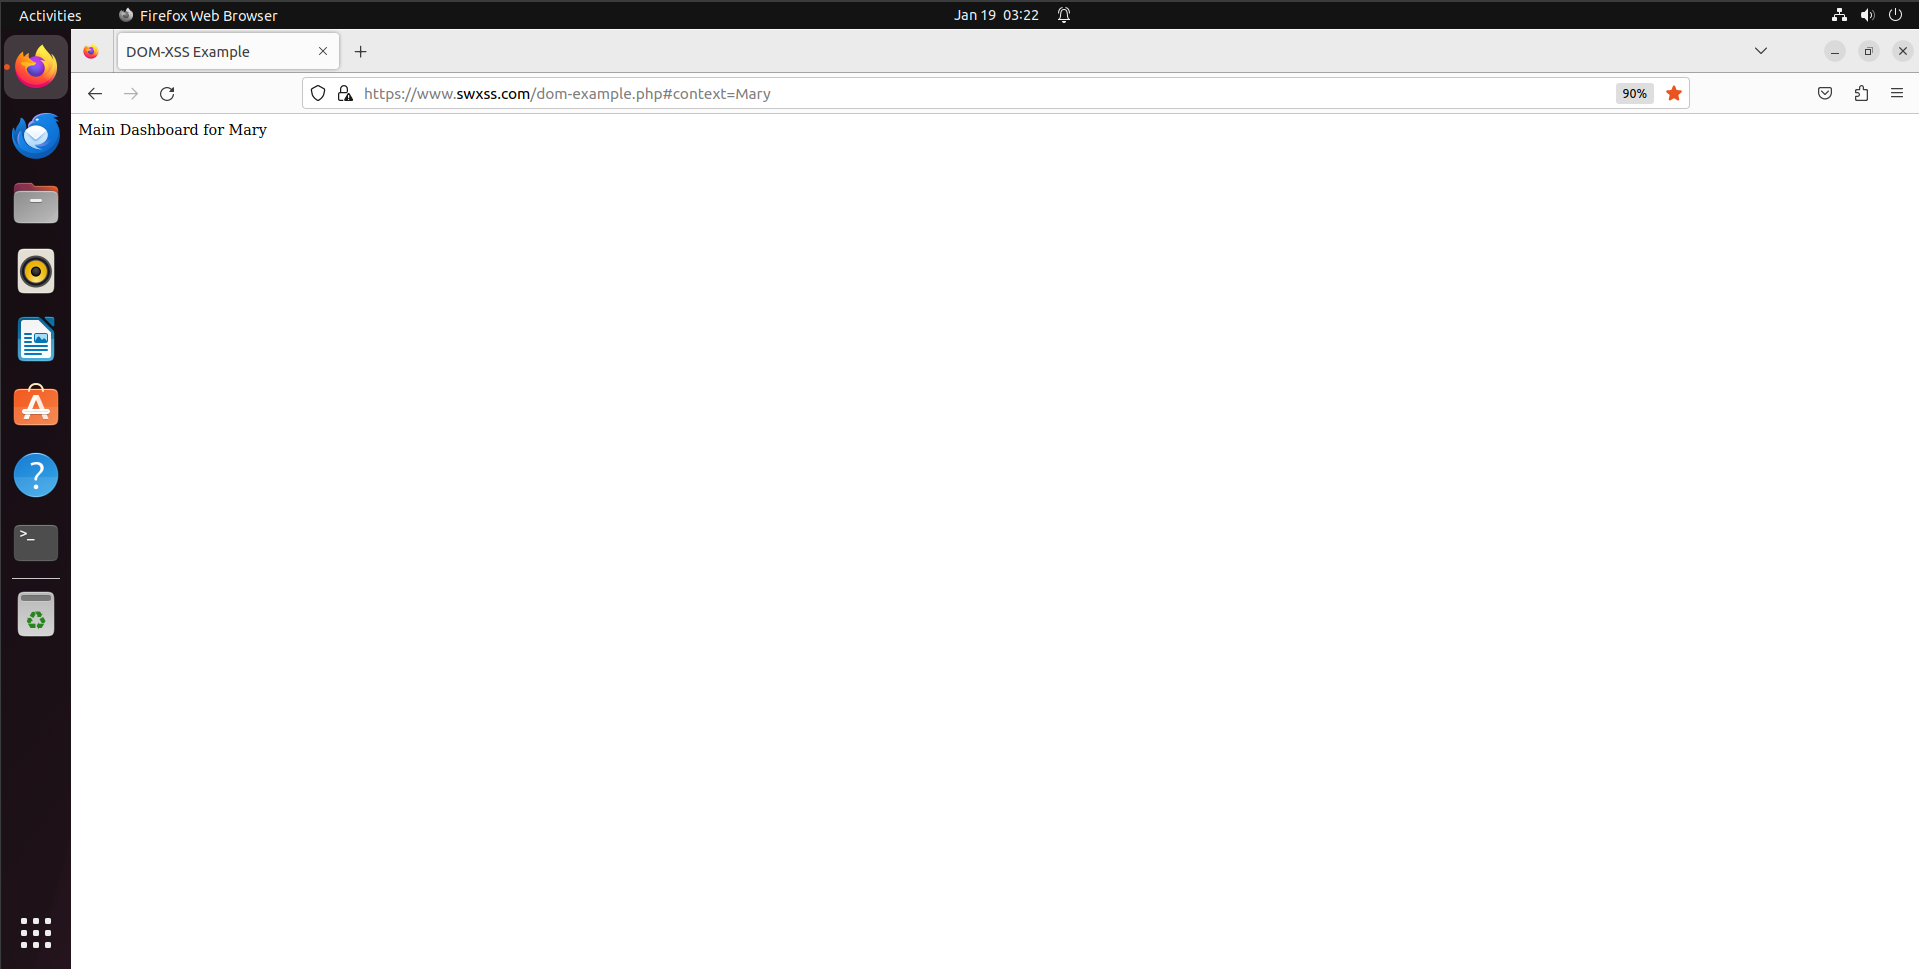
\includegraphics[width=0.75\linewidth]{graphics/verify-success.png}
        \caption{Success!}
        \label{fig:verify-success}
    \end{figure}
    
    \item The most likely culprit of the attacker not being able to see the website is the internal network not importing correctly. If one or both of the images are not on the same internal network---as seen in Figure~\ref{fig:verify-network}---then the website cannot be reached. To put both machines on the same network, first shut down both virtual machines. Once both machines are shut down, select one of them and open the settings (Figure~\ref{fig:fix-open-settings}). Once the Settings for the machine has been opened, navigate to the Network menu (Figure~\ref{fig:fix-settings-network}). For each adapter after Adapter 1 in the Network menu, uncheck the ``Enable Network Adapter'' checkbox (Figure~\ref{fig:fix-network-disable}). For Adapter 1, make sure the ``Enable Network Adapter'' checkbox is checked and change the ``Attached to:'' option to ``Internal Network'' (Figure~\ref{fig:fix-network-attached}). Finally, change the name of the internal network to ``swxss-network'' (Figure~\ref{fig:fix-network-name}). Repeat this process for the other machine and then go back to Step 1. If issues persist, please reach out to Dylan Gresham (dylangresham@u.boisestate.edu).

    \begin{figure}[!htbp]
        \centering
        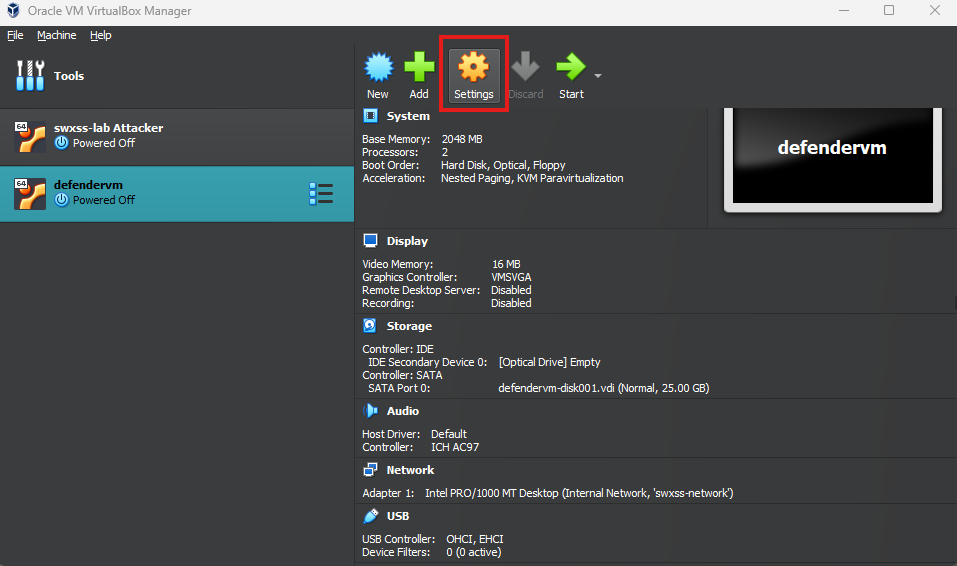
\includegraphics[width=0.75\linewidth]{graphics/fix-open-settings.png}
        \caption{Open settings for a virtual machine.}
        \label{fig:fix-open-settings}
    \end{figure}
    
    \begin{figure}[!htbp]
        \centering
        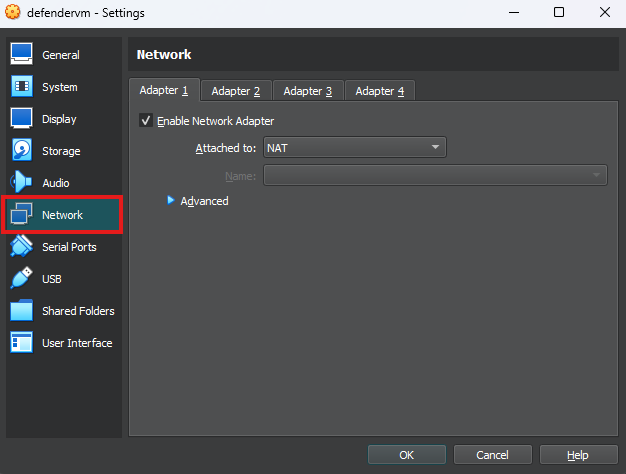
\includegraphics[width=0.75\linewidth]{graphics/fix-settings-network.png}
        \caption{Open the Network settings for a virtual machine.}
        \label{fig:fix-settings-network}
    \end{figure}
    
    \begin{figure}[!htbp]
        \centering
        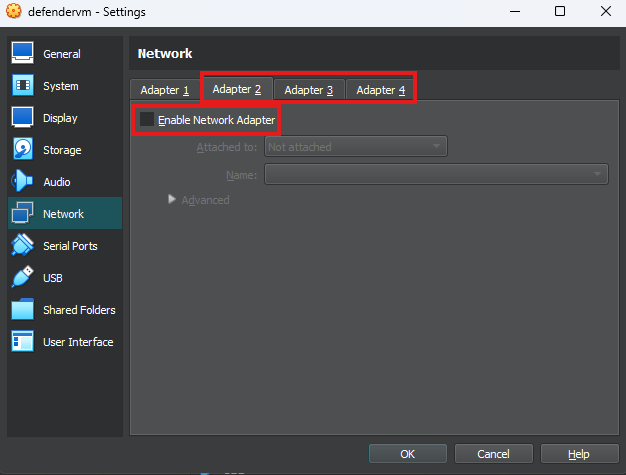
\includegraphics[width=0.75\linewidth]{graphics/fix-network-disable.png}
        \caption{Disable network adapters 2, 3, and 4.}
        \label{fig:fix-network-disable}
    \end{figure}
    
    \begin{figure}[!htbp]
        \centering
        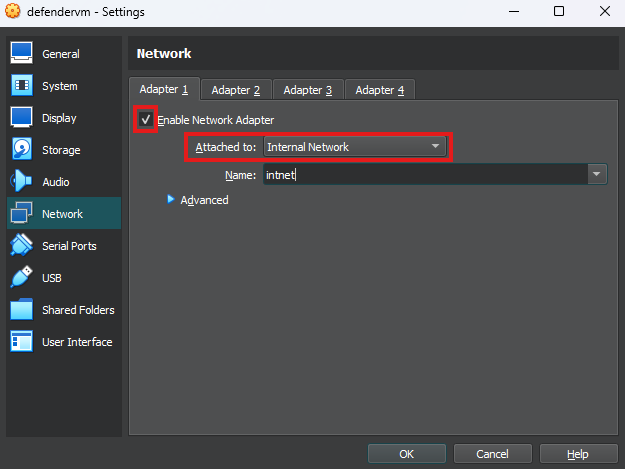
\includegraphics[width=0.75\linewidth]{graphics/fix-network-attached.png}
        \caption{Change Adapter 1 to attach to an Internal Network (name of network may vary).}
        \label{fig:fix-network-attached}
    \end{figure}
    
    \begin{figure}[!htbp]
        \centering
        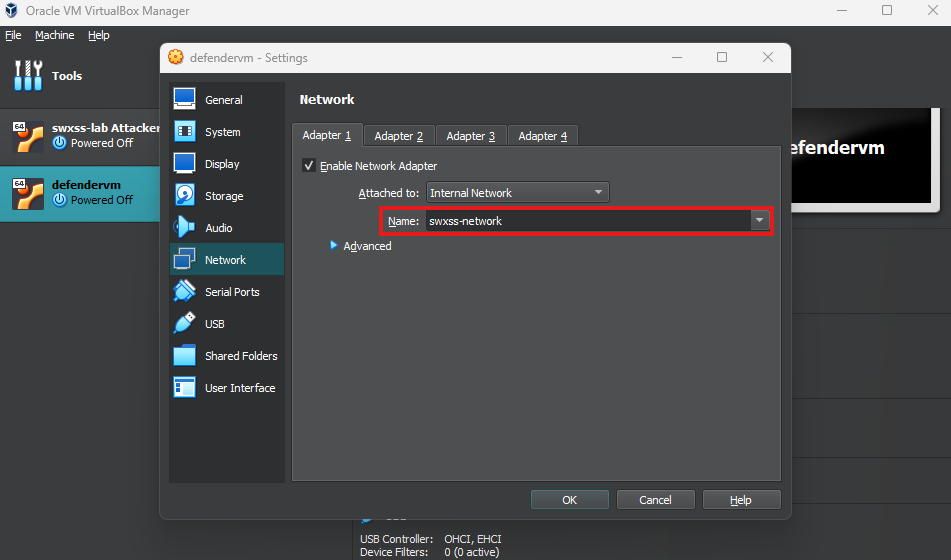
\includegraphics[width=0.75\linewidth]{graphics/fix-network-name.png}
        \caption{Change name of the internal network.}
        \label{fig:fix-network-name}
    \end{figure}
    
    \item Congratulations, you've successfully imported both virtual machine images and are now ready for the Web Security workshop segment of the BEACON Labs Workshop. Thank you for coming prepared! If you haven't already, please follow the instructions for the Network and Mobile Security material setups. We look forward to seeing you in Boise for the workshop!
\end{enumerate}

\end{document}

%%%%%%%%%%%%%%%%%%%%%%%%%%%%%%%%%%%%%%%%%